\section{The Basics of Counting}

\begin{definition}[The Product Rule]{def5.1:label}
    Suppose that a prodecure can be broken down into a sequence of two tasks (task 1 then task 2). If there are $n_1$ ways to do the first task and $n_2$ ways to do the second task following the first task, then tehre are $n_1\cdot n_2$ ways to do the procedure.
\end{definition}

\begin{problem}
    a) How many two letter strings can be made from the letters from the set $S \{A,B,C\}$?\\

    \begin{itemize}
        \item $AA,AB,AC$
        \item $BA,BB,BC$
        \item $CA,CB,CC$
    \end{itemize}

    Therefore there are a total of 9 ways that two letter strings can be made from the elements of the set $S$. Notice how the first choice was counting the "rows" and the second choice was counting the "columns."\\

    b) What happens if the letters cannot be repeated?

    \begin{itemize}
        \item $AB,AC$
        \item $BA,BC$
        \item $CA,CB$
    \end{itemize}

    Therefore there are a total of 6 ways that two letter strings without letter repeats can be made from the elements of the set $S$. Notice again how the first choice was counting the "rows" and the second choice was counting the "columns."
\end{problem}

\begin{problem}
    A multiple choice exam contains 10 questions. There are four possible answers for each question.\\

    \textbf{1) How many ways can a student answer the questions if every question is answered?} $4^10$

    \textbf{2) H}
\end{problem}


\begin{definition}[The Sum Rule]{def5.2:label}
    Suppose that there are $n_1$ ways to do task 1 and $n_2$ ways to do task 2. If thereis no overlap between the two tassk, then there are $n_1+n_2$ ways to do either task 1 OR task 2 (this means that task 1 and task 2 must be independent of each other).
\end{definition}

\begin{problem}
    A class has 4 freshman, 6 sophomores, 3 juniors, and 5 seniors. An upper-classmen must be selected to represent the class. 
    
    \textbf{In how many ways can this be done?:} $3 + 5 = 8$ total ways to do this.\\

    \textbf{How many bit strings are there of length 4 or less?:} $2 + 2^2 + 2^3 + 2^4$\\
\end{problem}

\begin{problem}
    How many license plates can be made with either 4 digits (0-9) followed by 2 letters (A-Z) or 3 digits followed by 3 letters?

    $$
    10^4 \cdot 36^2 + 10^3 \cdot 26^3
    $$
\end{problem}


\begin{definition}[Principle of Inclusion-Exclusion]{def5.3:label}
    Suppose that there are $n_1$ ways to do task 1 and $n_2$ ways to do task 2, and $k$ ways to do both. Then there are $n_1+n_2-k$ ways to do task 1 or task 2.
\end{definition}

\begin{problem}
    How many positive integers less than 100\dots

    \begin{itemize}
        \item Are divisible by 5? \textbf{19}
        \item Are divisble by 3? \textbf{33}
        \item Are divisble by both 3 and 5? \textbf{6}
        \item Are divisible by either 3 or 5? $19+33-6$ = \textbf{46}
        \item Are divisble by excactly one of 3 and 5? $46-6$ = \textbf{40}
        \item Are divisible by neither 3 nor 5? $100 - 46$ = \textbf{53}
        \item Are divisible by 3, but not 5? $33-6$ = \textbf{27}
    \end{itemize}
\end{problem}



\section{The Pigeonhole Principle}

\begin{definition}[The Pigeonhole Principle]{def5.2.1:label}
    Suppose that $k$ is a positive integer and $k+1$ or more obkects are placed into $k$ boxes, then at least one box contains two or more objects.
\end{definition}

\begin{problem}
    In a room of 16 people, we know that at least two were born in the same month. What are the 'boxes' and what are the 'objects'?\\

    \textbf{BOXES:} the months of the year
    \textbf{OBJECTS:} the people that are in the room
\end{problem}


\begin{definition}[The GENERALIZED Pigeonhole Principle]{def5.2.2:label}
    Suppose that $N$ is a positive integer and $N$ objects are place in $k$ boxes. Then at least one box contains at least $N/k \text{ CEILING FUNCTION}$.
\end{definition}


\begin{problem}
    In a room of 16 people, at least how many were born on the same day of the week? (16/7 then round up).
\end{problem}



\section{Permutations and Combinations}

\begin{definition}{def6.3:label}
    A \textbf{permutation} without repetition of a set of objects is an ordered arrangement of the objects. An \textbf{$r$-permutation} without repetition is an ordered arrangement of $r$ elements of a set. 
\end{definition}


\begin{problem}
    Let $S=\{a,b,c\}$

    \begin{itemize}
        \item List all of the permutations of $S$.
        \begin{itemize}
            \item abc, bca, cba, acb, bac, cab
        \end{itemize}
        \item List all of the 1-permutations of $S$.
        \begin{itemize}
            \item a,b,c
        \end{itemize}
        \item List all of the 2-permutations of $S$.
        \begin{itemize}
            \item ab, bc, cb, ac, ba, ca
        \end{itemize}
    \end{itemize}
\end{problem}


\begin{theorem}{theorem5.3:label}
    If $n$ is a positive integer and $r$ is an integer between 1 and $n$ (inclusive), then there are:

    $$
    P(n,r) = n(n-1)(n-2)\cdots(n-r+1) = \frac{n!}{(n-r)!}
    $$

    $r$-permutations of a set with $n$ distinct elements.
\end{theorem}


\textbf{NOTE:} There are some following unique applications of this theorem to keep in mind:

\begin{itemize}
    \item $P(n,0) = 1$ which corresponds to "one way to order zero elements"
    \item $P(n,n) = n!$ which corresponds to "$n!$ was to order $n$ elements"
\end{itemize}


\begin{problem}
    An Olympic 200m finals has 8 runners.

    \begin{itemize}
        \item In how many ways can the runners finish assumin no ties? $P(8,8) = 8!$
        \item In how many ways can Gold, Silver, and Bronze be awarded assuming no ties? $P(8,3) = frac{8!}{5!}=8\cdot 7\cdot 6$
        \item How many different sets of 3 medalists are there in a race with 8 runners?
    \end{itemize}
\end{problem}


\begin{definition}{def5.3.2:label}
    An \textbf{$r$-combination} (without repetition) of a set of $n$ objects is an unordered selection of $r$ of the objects from the set.
\end{definition}


\begin{theorem}{theorem5.3.2:label}
    If $n$ is a non-negative integer and $r$ is an integer between 0 and $n$ (inclusive), then there are 
    
    $$
    C(n,r) = \frac{P(n,r)}{r!}
    $$

    $r$-combinations in a set of $n$ elements.
\end{theorem}


\section{Binomial Coefficients and Identities}

Check out this pattern:

\begin{itemize}
    \item $(x+y)^0 = 1$
    \item $(x+y)^1 = x+y$
    \item $(x+y)^2=x^2+2xy+y^2$
    \item $(x+y)^3=x^3+3x^2y+3y^2x+y^3$
\end{itemize}

\begin{definition}[The Binomail Theorem]{def5.4.1:label}
    Let $x$ an $y$ be variables and $n$ be a non-negative integer. Then:

    $$
    (x+y)^n = \sum_{k=0}^n n()kx^ky^{n-k}
    $$
\end{definition}

\begin{problem}
    Expand $(x+y)^5$

    $$
    \begin{aligned}
        (x+y)^5 &= (x+y)(x+y)(x+y)(x+y)(x+y)\\
        &= 5()5x^5+5()4x^4y+5()3x^3y^2+5()2x^2y^3+5()1xy^4+5()0y^5\\
        &= x^5+5x^4y+10x^3y^2+10x^2y^3+5xy^4+y^5
    \end{aligned}
    $$
\end{problem}

\begin{center}
    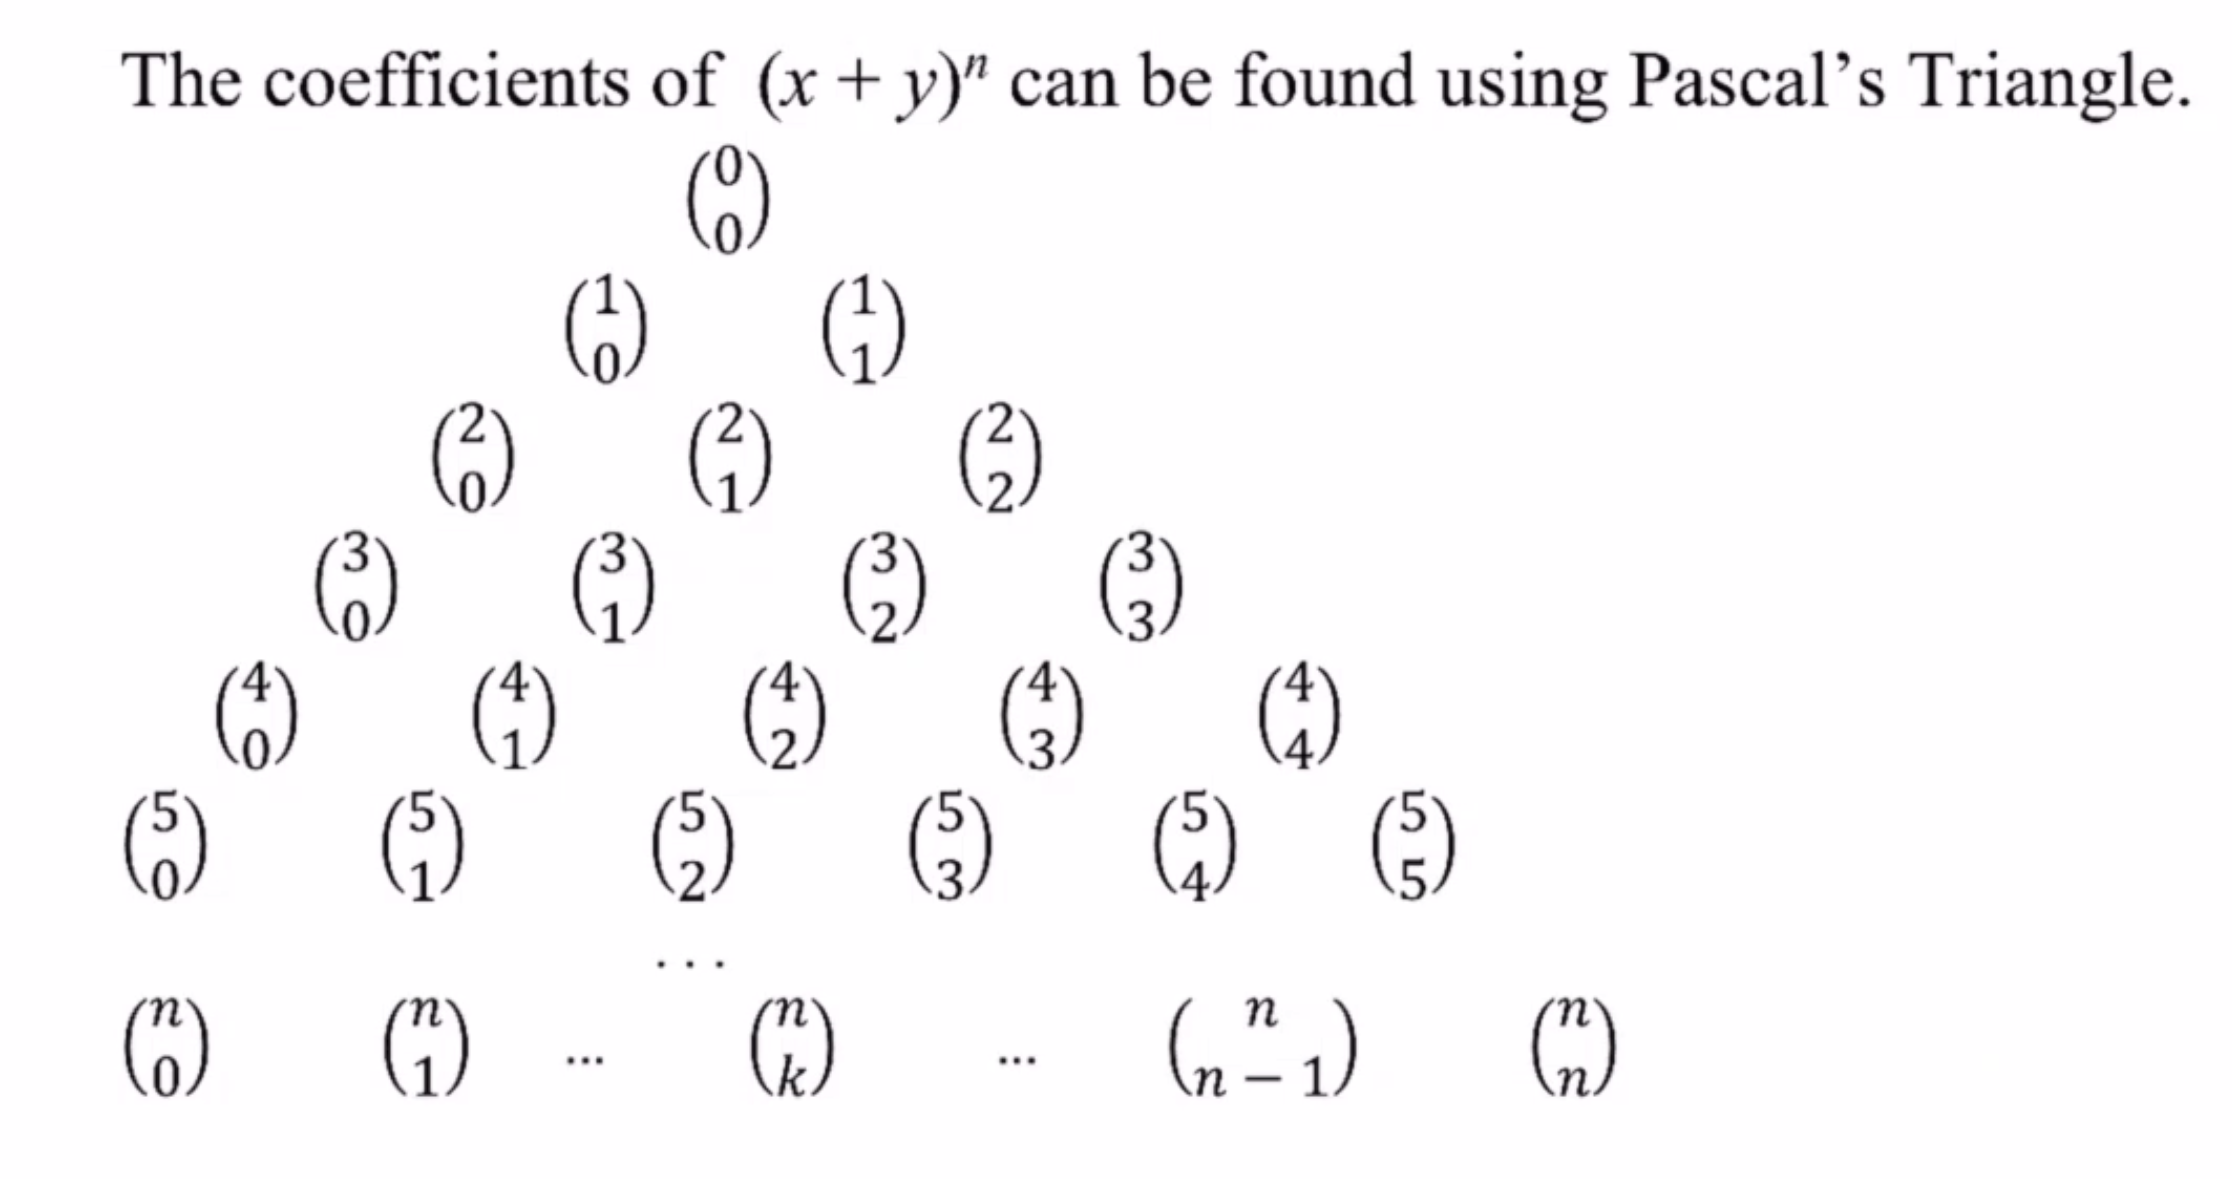
\includegraphics[width=1\textwidth]{chapters/ch5/images/fig5.4.1.PNG}
\end{center}